\subsection{C-RNN analysis}

\begin{table*}[htbp]
\centering
    \begin{tabular}{c  c  c   c  c }  
        \toprule
        Split & MAE & NLL & $\mathcal{A}$ & $\mathcal{E}$\\
        \midrule
        Test & 0.55(1, 0.09) & 0.44(1.5, -0.7) & 0.62(1.15, 0.09) &  -4.6\\
        OOD  &  2.6(4.9, 0.29) &  17.8(31.2, 4.48) & 0.61(1.12, 0.09)&  -0.25\\
        \midrule
    \end{tabular}
    \caption[Revs C-RNN performance]{Revs C-RNN performance. $\mathcal{E}$ is the average epistemic uncertainty, and $\mathcal{A}$ the average aleatoric uncertainty}
    \label{tbl:revs}
\end{table*}

We start by looking at the results of our C-RNN model, \cref{fig:Revs_run} shows plots for one test and one OOD sample from the revs dataset. Each plot shows both the longitudinal and lateral velocities, along with the model's predictions and uncertainties.
We can see that errors go up for the OOD input compared to the test input. The overlayed green shading in the plot represents the epistemic uncertainty, and we can see from comparing the two plots that the epistemic uncertainty is higher for the OOD sample. The epistemic uncertainty is also plotted below the main plot, to show the numerical values. For a more concrete view, we look at the numbers.

\Cref{tbl:revs} contains the MAE, NLL, and the average uncertainties for the test and OOD splits. There we can see the MAE go from 0.55 for the test data to 2.6 for the OOD data, roughly a fivefold increase. The NLL goes from 0.44 to 17.8, a roughly forty fold increase. This sharp increase in the NLL suggests that not only does the MAE go up, but also that the aleatoric uncertainty does not go up enough to match it. Indeed the aleatoric uncertainty is roughly the same for both splits, despite the large increase in errors. 
Recall that the aleatoric uncertainty is the scale of the Gaussian representing the model's belief. We suspect that the model systematically outputs overly narrow Gaussians for the OOD data, and that this is a contributing factor in the sharp rise of the NLL.  
We clarify this intuition with a simple experiment. We can manually increase the model's aleatoric uncertainty, and check whether this improves the NLL. We simply add a constant(0.5) to the $\sigma_y$ the model outputs, and the NLL for the OOD data goes down from 17.8 to 5.12, for the test data the NLL goes up, from 0.44 to 1.03.

The epistemic uncertainty, on the other hand, increases from -4.6 to -0.25, confirming that the trend we saw in \cref{fig:Revs_run}.

% \begin{figure}[htbp]
%   \centering
  
%   \begin{subfigure}[b]{\textwidth}
%     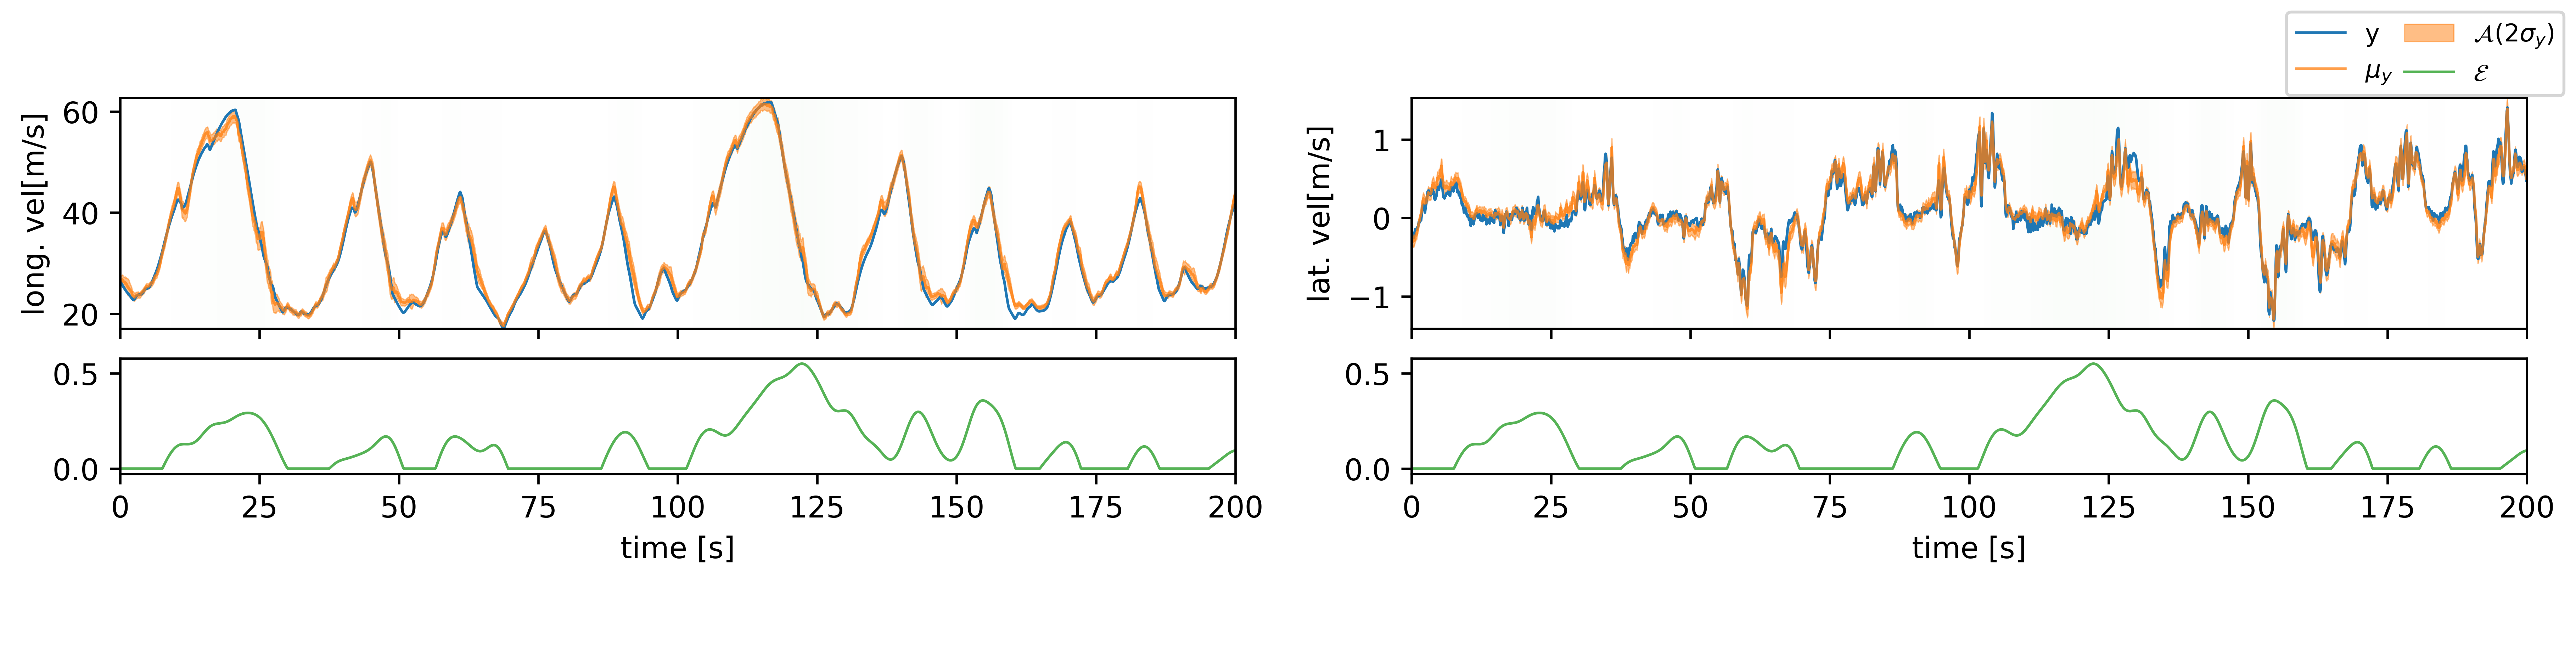
\includegraphics[width=\textwidth]{Experiments/figs/revs_test.png}
%     \caption{Test}
%   \end{subfigure}
  
%   \begin{subfigure}[b]{\textwidth}
%     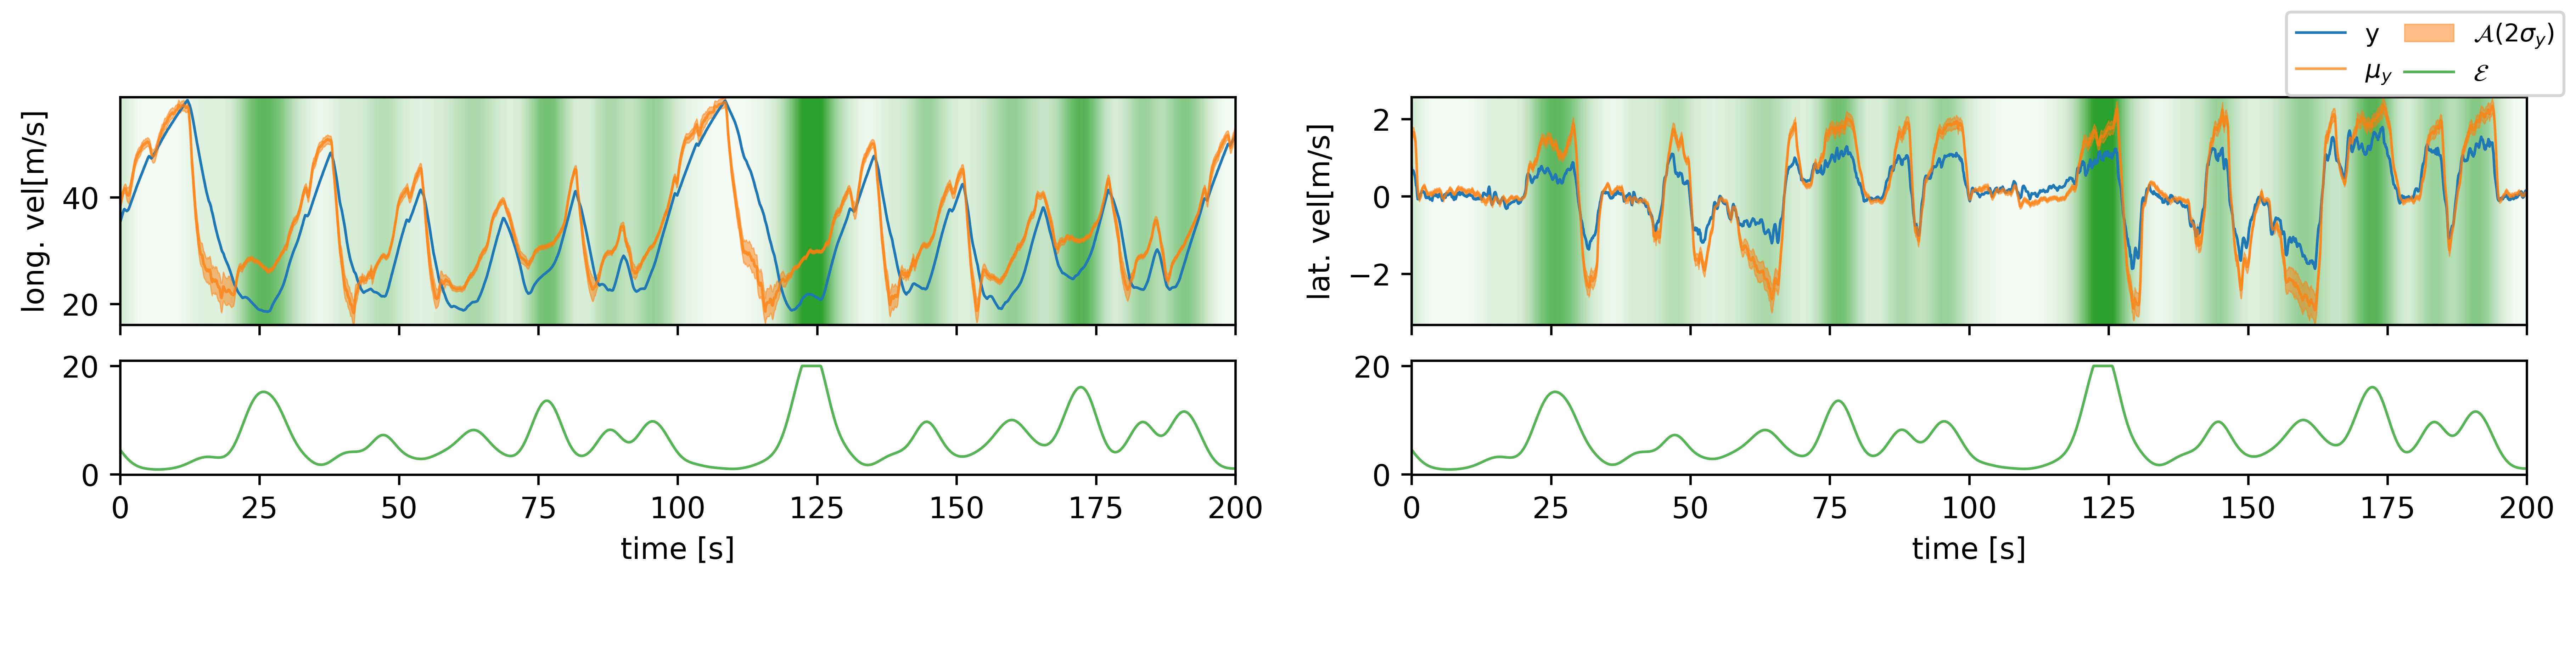
\includegraphics[width=\textwidth]{Experiments/figs/revs_ood.png}
%     \caption{OOD}
%   \end{subfigure}
  
%   \caption[Revs prediction plots for C-RNN]{Revs test and ood plots for C-RNN. Aleatoric uncertainty represented as the shaded interval around the prediction(1 std on each side). Epistemic Uncertainty plotted in the bottom row. The green shading also represents the epistemic uncertainty overlayed over the graph. The green shading has the same scaling for the test and OOD plots.}
%   \label{fig:Revs_run}
% \end{figure}


Those results are consistent with the expectations we formulated in \cref{ch:background}. It may seem surprising to some that the average aleatoric uncertainty does not go up at all over the OOD data, but as we said in \cref{subsec:aleatoric} model learns to estimate aleatoric uncertainty from the training data. In this light, it is not shocking that the average behavior does not change much across input regions. The model seems to be simply matching the statistics it learned during training. 

This motivated our design for C-RNN, which explicitly models the training distribution. We can see empirically that C-RNN succeeds at assigning high uncertainty to OOD inputs where the errors are high.   


\begin{table*}[htbp]
\centering
    \begin{tabular}{c  c  c}  
        \toprule
        Uncertainty score & AUROC$\uparrow$ & FPR@95\%$\downarrow$\\
        \midrule
        Aleatoric($\mathcal{A}$) & 0.47  & 0.90\\
        Epistemic($\mathcal{E}$) & 0.97 &  0.05 \\
        \midrule
    \end{tabular}
    \caption[Revs OOD discrimination power for C-RNN]{Revs OOD discrimination power of the aleatoric($\mathcal{A}$) and epistemic($\mathcal{E}$) uncertainties for C-RNN.}
    \label{tbl:revs_discrimination}
\end{table*}


\begin{table*}[htbp]
\centering
    \begin{tabular}{l l c c c c}  
        \toprule
        U. & Split & \multicolumn{2}{c}{MAE} & \multicolumn{2}{c}{$Zs$}\\
        \midrule
        & & $\rho \uparrow$ & $r \uparrow$ & $\rho \uparrow$ & $r \uparrow$ \\
        \multirow{3}{*}{$\mathcal{A}$} 
            & Test     & 0.57(0.51, 0.63) & 0.58(0.53, 0.62) & - & - \\  
            & OOD      & 0.49(0.36, 0.82) & 0.5(0.17, 0.83) & - & - \\  
            & Test+OOD & 0.39(0.16, 0.62) & 0.3(0.05, 0.54) & - & - \\ 

        \midrule
        \multirow{3}{*}{$\mathcal{E}$} 
            & Test     & 0.32  & 0.34 &  0.23  & 0.19 \\  
            & OOD      & 0.57 & 0.61 &  0.88 & 0.86 \\
            & Test+OOD & 0.85 & 0.80 &  0.93 & 0.91 \\ 

        \toprule
    \end{tabular}
    \caption[Revs uncertainty-error correlations for C-RNN]{Pearson $\rho$ and Spearman $r$ correlations between the uncertainties and error scores. In the top half we check correlations with Aleatoric uncertainty, and in the bottom half with the epistemic uncertainty.}
    \label{tbl:revs_corr}
\end{table*}


To see how well our uncertainties can discriminate between the in/out-of-distribution data, we use to the AUROC and FPR@95\% metrics. \cref{tbl:revs_discrimination} shows the results of those metrics when we use either the aleatoric or epistemic uncertainty to discriminate between test/OOD inputs. The results clearly show that the epistemic uncertainty does an excellent job at separating the two splits. The AUROC has a maximum of 1, and represents the probability that a random test input has lower uncertainty that a random OOD input. C-RNN's epistemic uncertainty puts that probability at 0.97. The aleatoric uncertainty is performing roughly on par with random behavior, which would have an expected 0.5 probability to give a test input lower score than an ood input.
To further understand the behavior and role of the uncertainties we need to look at correlations between errors and uncertainties. 


\Cref{tbl:revs_corr} shows the correlations between our error scores and uncertainties. The table is split such that the top half contains correlations between the errors and aleatoric uncertainty, and the bottom half between the errors and the epistemic uncertainty. For each uncertainty, we look at the correlations over the test and OOD splits separately, then combined.  

The aleatoric uncertainty shows the strongest correlations with the MAE over the test split alone, with an 0.57 Pearson coefficient. Within the OOD split alone the aleatoric uncertainty still shows good correlation with the MAE, with a Pearson correlation of 0.49. However, over the combined splits, the correlation drops to 0.39. Given the fact that the average aleatoric uncertainty does not change between the test and OOD splits, while the MAE increases fivefold, it is not surprising that the correlation over the combined splits is low. 

The epistemic uncertainty shows the reverse behavior for its correlation with the MAE, having the highest correlation over the combined splits with a Pearson coefficient of 0.85. More notably, the epistemic uncertainty correlates strongly with the Z-score. We can see that it correlates weakly with the Z-score over the test split, correlates better over the OOD split, and best over the combined splits with a Pearson coefficient of 0.93. The Z-score increases as the ratio of the MAE to the epistemic uncertainty increases. 

Those results suggest that our model uncouples the uncertainties, to an extent, and each uncertainty is playing the role we expected. The aleatoric uncertainty focuses on errors within the test data, and the epistemic uncertainty focuses on errors coming from the OOD data. 

\Cref{fig:revs_uncertainty_corr} shows binned diagonal plots of the uncertainties versus our error scores over the combined splits. In those plots we perform quantile binning of the points according to the error score, then we plot the uncertainty over the quantiles of the error. The error bars in the plot represent the standard deviation of the uncertainty within each quantile. We use the MAE, Z-score, and the NLL as error scores. 

The plots show a roughs separation of the points into a cluster of in-distribution low error bins and a tail of OOD high error points. We can see from \cref{fig:revs_epistemic_corr} that as we move away from the cluster of low error points the epistemic uncertainty increases steadily.   

The situation with the aleatoric uncertainty is complicated. We should again note that the aleatoric uncertainty is used in the calculation of both the NLL and the Z-score, as such we only include those plots for completeness, but we cannot offer a meaningful interpretation. Our focus for the aleatoric uncertainty is to observe its relationship with the MAE. We can see that for the low MAE points, the aleatoric uncertainty shows a correlation, but as we move farther into higher error OOD bins, the correlation \emph{restarts}. Looking at the center plot of \cref{fig:revs_aleatoric_corr}, we can see that the aleatoric uncertainty correlates with the MAE separately within the low error in-distribution bins, and within the high error OOD region.
This is consistent with the numbers we see in \cref{tbl:revs_corr}, where we see that the correlation between aleatoric uncertainty and MAE is higher within the individual splits than when looking at the combined splits.

\begin{figure}[htbp]
  \centering
    \begin{subfigure}[b]{\textwidth}
        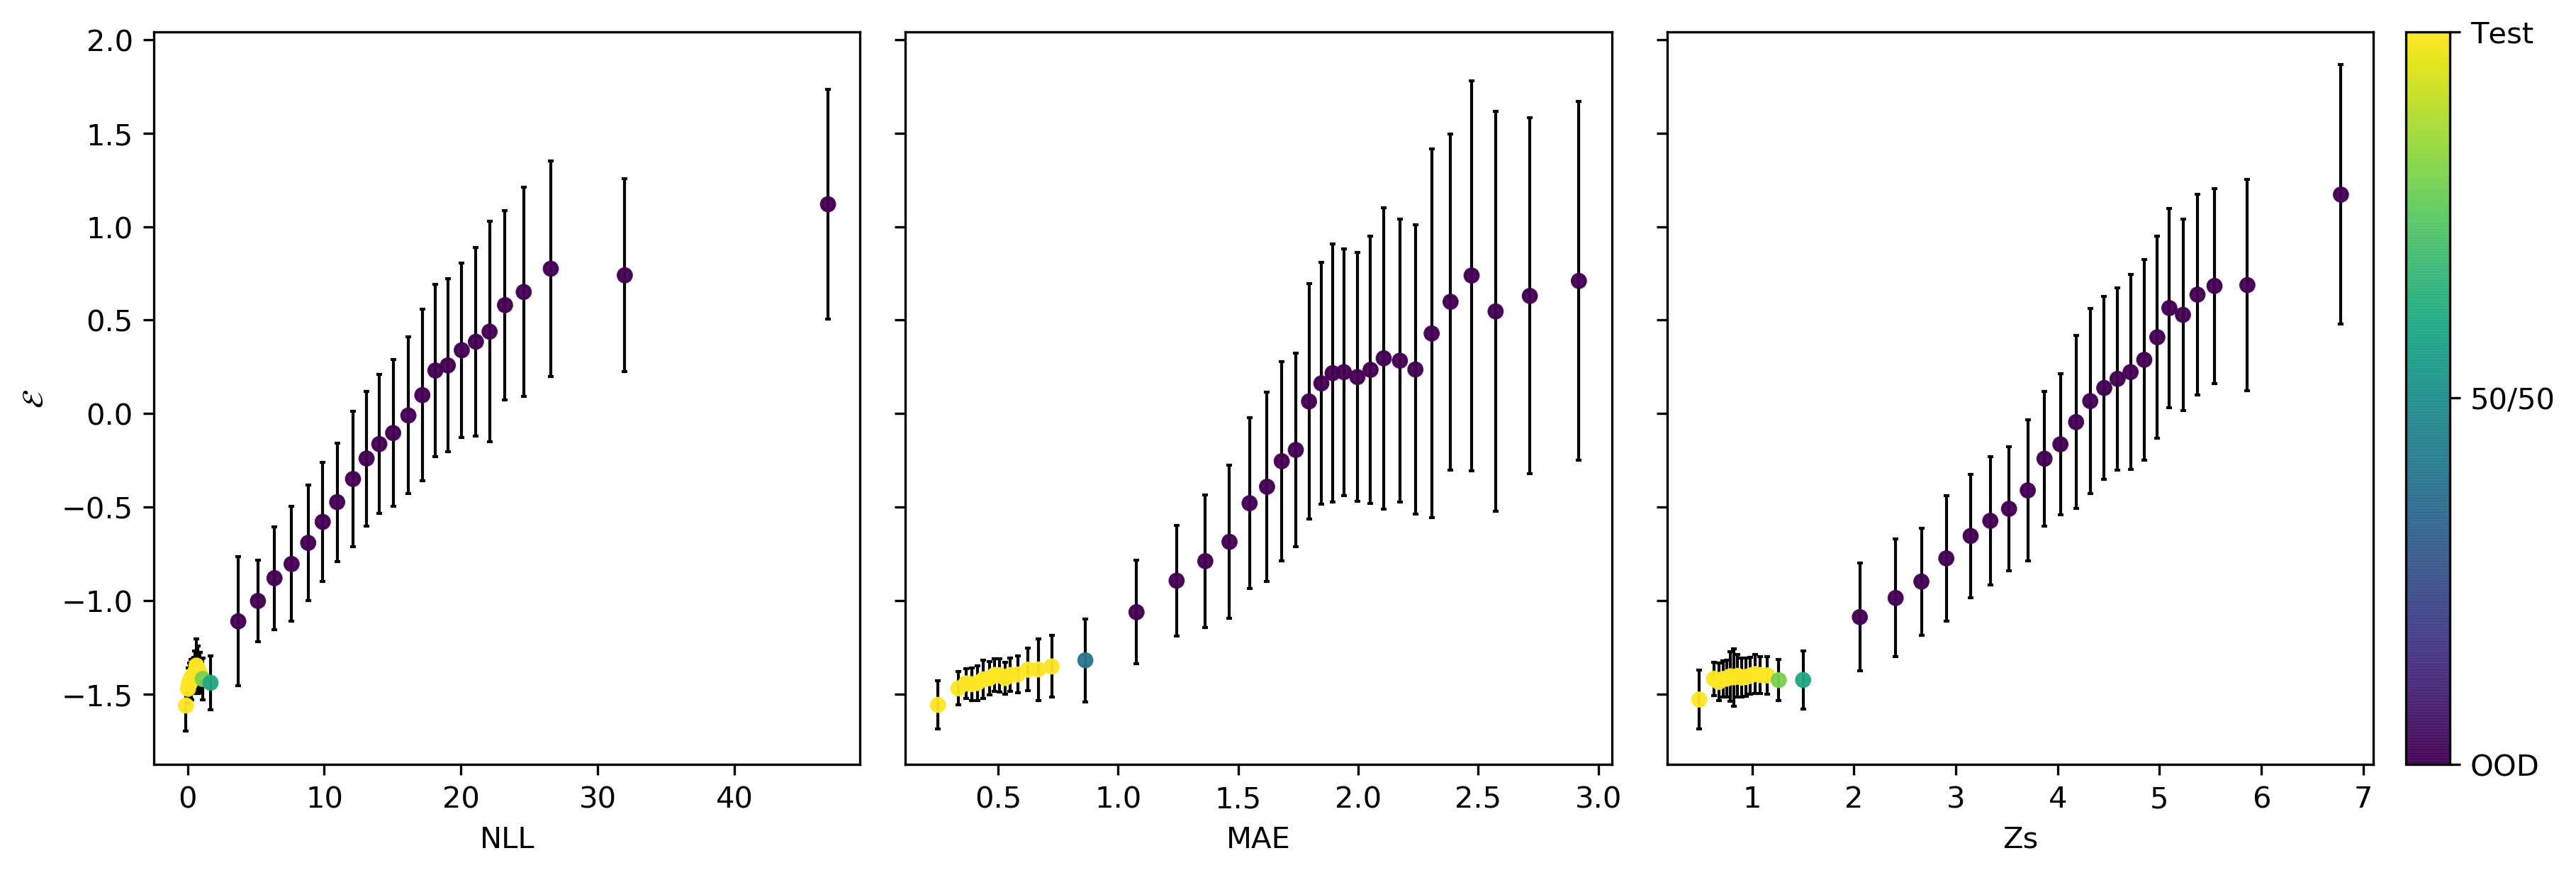
\includegraphics[width=\textwidth]{Experiments/figs/binned/revs_crnn_epistemic.png}
        \caption{Binned diagonal plots for the epistemic uncertainty.}
        \label{fig:revs_epistemic_corr}
    \end{subfigure}
    
    \begin{subfigure}[b]{\textwidth}
        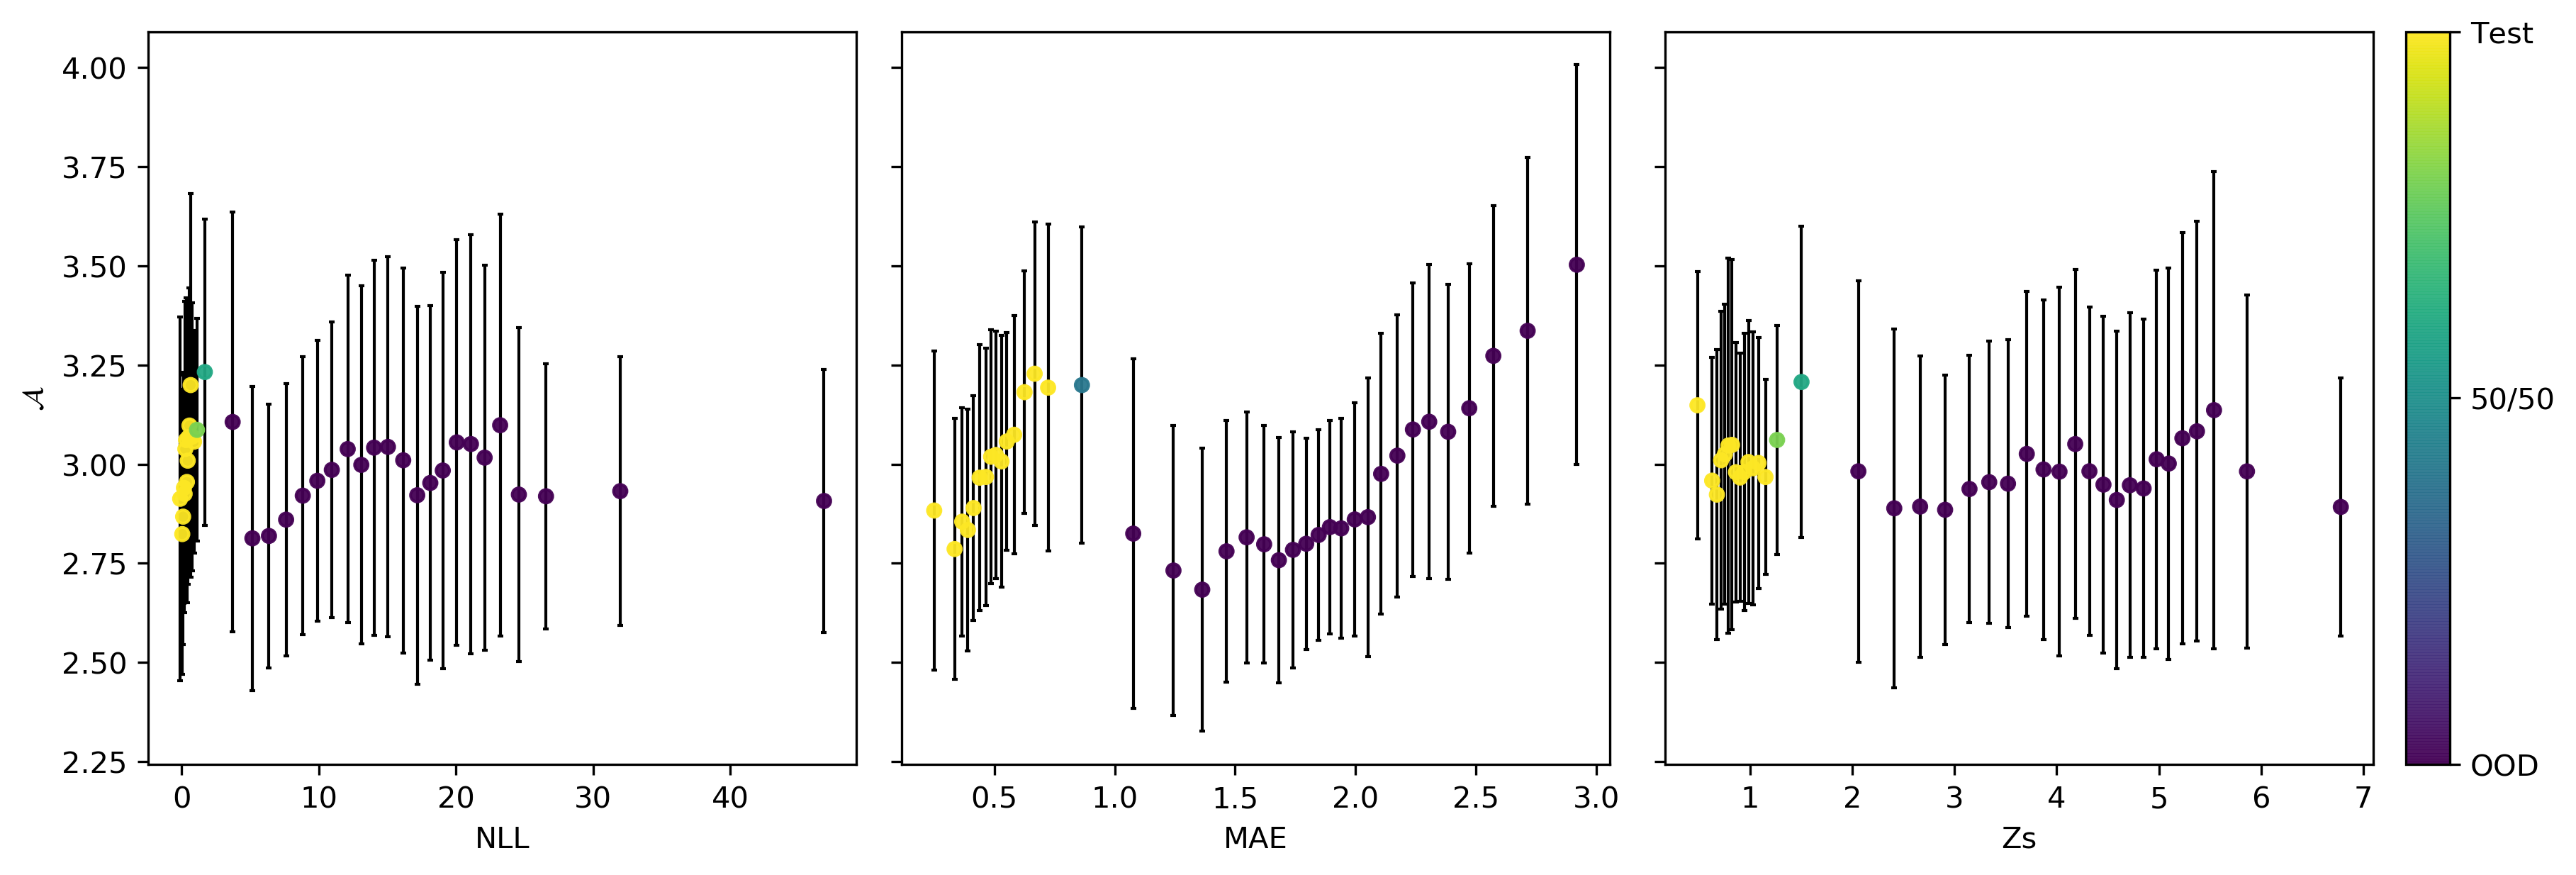
\includegraphics[width=\textwidth]{Experiments/figs/binned/revs_crnn_aleatoric.png}
        \caption{Binned diagonal plots for the aleatoric uncertainty.}
    \label{fig:revs_aleatoric_corr}
  \end{subfigure}
    \caption[Revs error-uncertainty diagonal plots for C-RNN]{Revs binned diagonal plots of the  uncertainty vs error scores(NLL, MAE, Z-score) over the combined splits(Test+OOD). The marker color denotes the ratio of test to OOD points in the bin. }
    \label{fig:revs_uncertainty_corr}
\end{figure}


Lastly we wish to explore the relationship between our two uncertainties. We compute the correlations between the epistemic and aleatoric uncertainties. For the combined splits(Test+OOD), we get a Pearson correlation of 0.01 between the aleatoric and epistemic uncertainty. For the test split only, we get a Pearson of 0.014. For the OOD split only, we get Pearson 0.39. Again suggesting that for the C-RNN model the two uncertainties play different roles. 

\clearpage
\subsection{What about Dropout?}

MC dropout~\citep{gal2016dropout} is widely used as a tool to estimate epistemic uncertainty in deep learning. We have trained dropout models to see their behavior in our context. We use MC dropout is a variational approximation to the bayesian approach discussed in \cref{ch:background}~\citep{gal2016dropout}. 

The dropout models we train estimate the aleatoric uncertainty identically to our models, via outputting the mean and variance of a Gaussian. Thus the main difference is in the epistemic uncertainty estimation. Note that our approach and dropout are more orthogonal than competing. They focus on different sources of uncertainty(cf. \ref{ch:background}) . Similar to the previous subsection, we will study the uncertainty dropout captures and how its two uncertainties interact with each other and the errors.

\begin{table*}[htbp]
\centering
    \begin{tabular}{c  c  c   c  c }  
        \toprule
        Split & MAE & NLL & $\mathcal{A}$ & $\mathcal{E}$\\
        \midrule
        Test &  1.26(2.4, 0.14) & 1.13(2.6, -0.37) & 2.38(4.5, 0.23) &  1.79(3.4, 0.14) \\
        OOD  &  2.55(4.9, 0.2)&  1.62(3.2, 0.02)& 2.42(4.6, 0.26)&  1.97(3.8, 0.16) \\
        \midrule
    \end{tabular}
    \caption[Revs MC dropout performance.]{Revs MC dropout performance. The numbers are given with their std}
    \label{tbl:revs_dropout}
\end{table*}


% \begin{figure}[htbp]
%   \centering
  
%   \begin{subfigure}[b]{\textwidth}
%     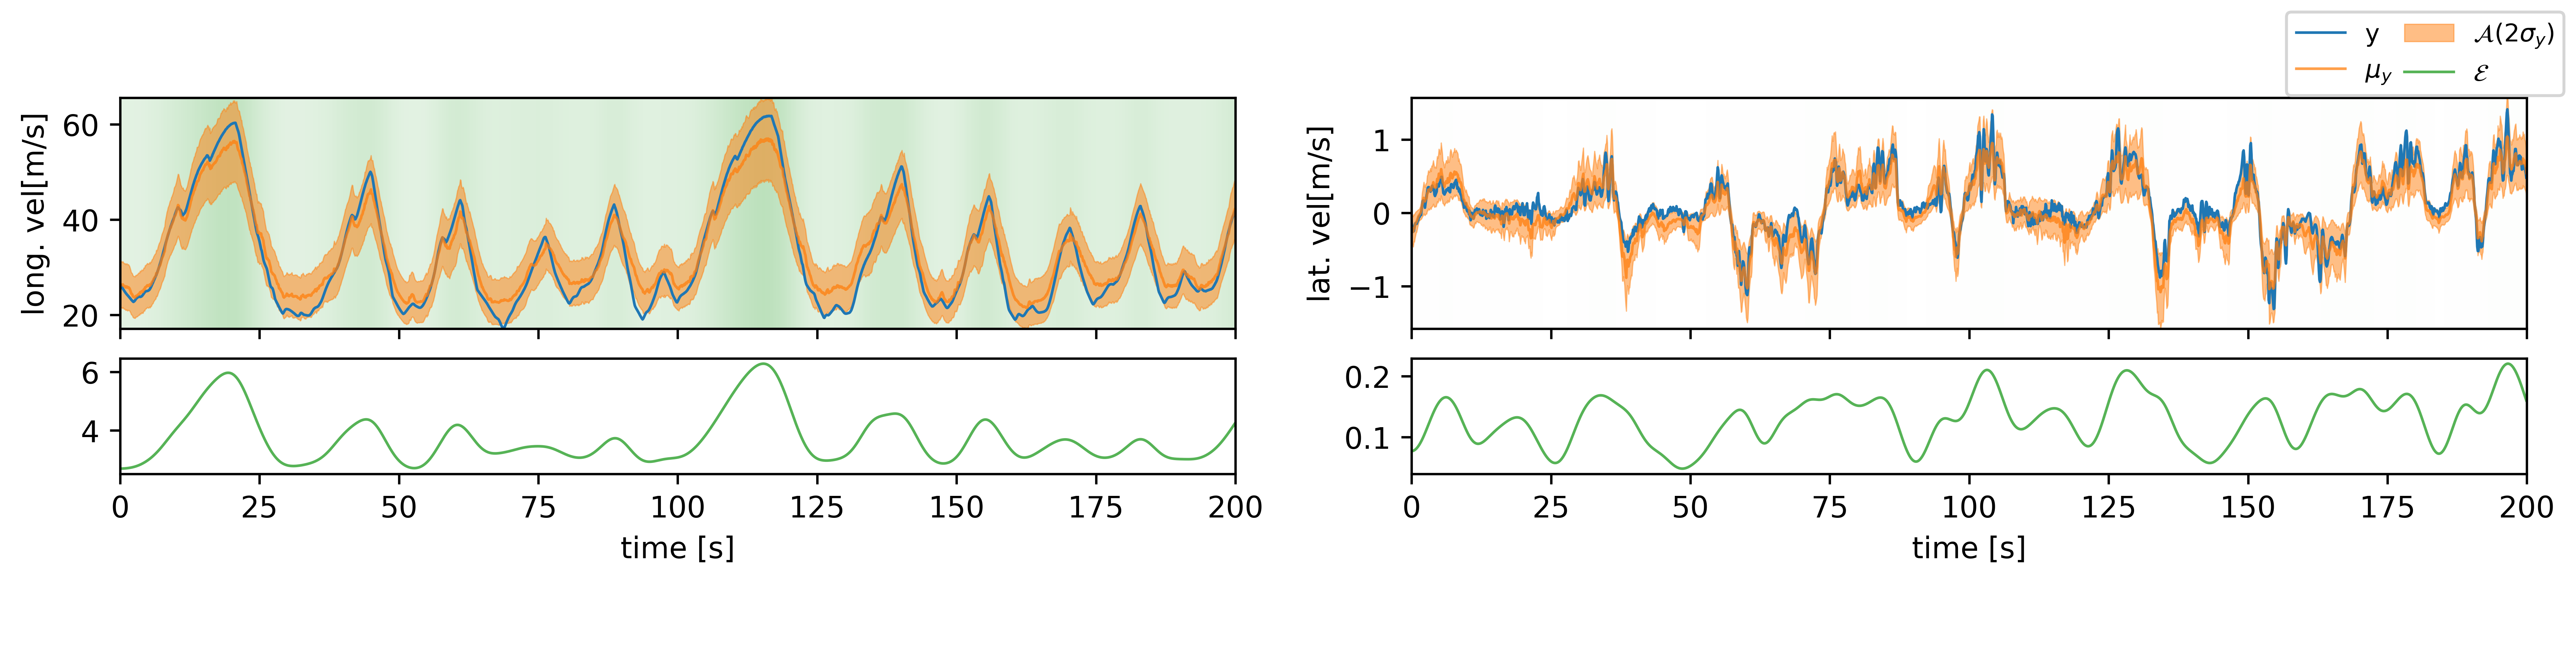
\includegraphics[width=\textwidth]{Experiments/figs/revs_dropout_test.png}
%     \caption{Test}
%   \end{subfigure}
  
%   \begin{subfigure}[b]{\textwidth}
%     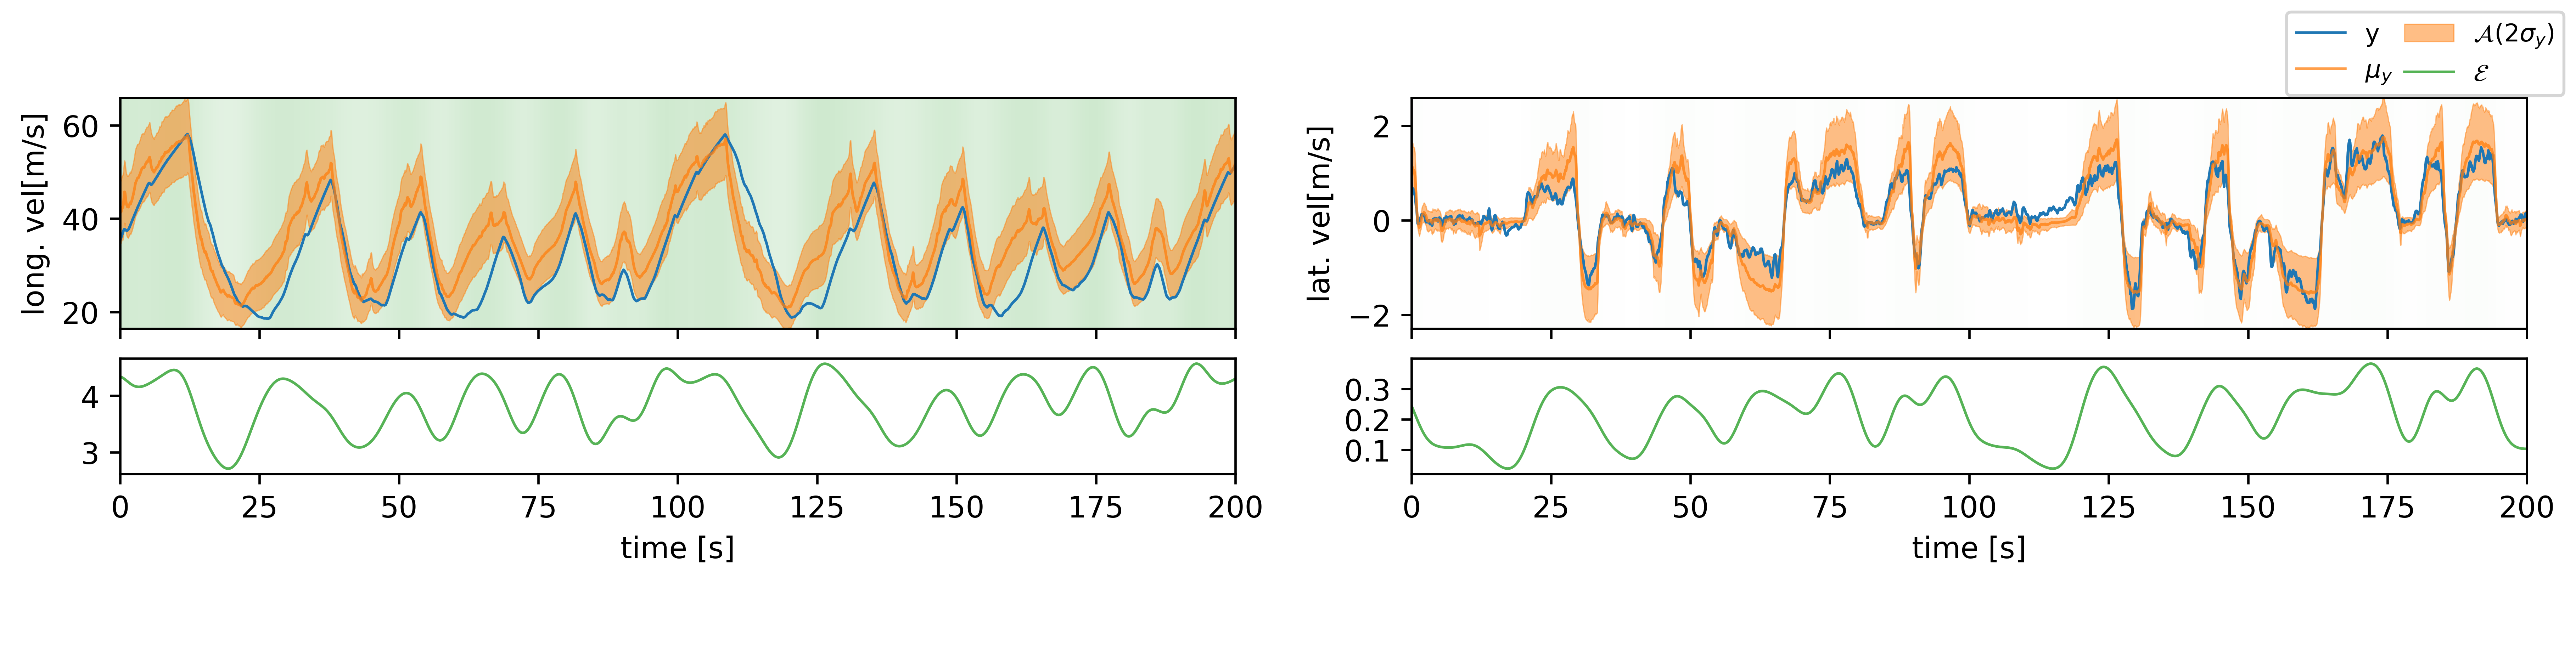
\includegraphics[width=\textwidth]{Experiments/figs/revs_dropout_ood.png}
%     \caption{OOD}
%   \end{subfigure}
  
%   \caption[Revs prediction plots for MC dropout]{Revs test and ood prediction plots for MC dropout. Aleatoric uncertainty represented as the shaded interval around the prediction(2 stds on each side). Epistemic Uncertainty plotted in the bottom row. The green shading also represents the epistemic uncertainty overlayed over the graph.}
%   \label{fig:revs_dropout_run}
% \end{figure}

\Cref{fig:revs_dropout_run} shows prediction plots for the dropout model. Again we see that the model performance decreases over the OOD input. Another important thing to notice is that the epistemic uncertainty lies in the same range for both the test and OOD input. We will look at the numbers.

\Cref{tbl:revs_dropout} shows the basic results of MC dropout. Again we see that the MAE is higher on the OOD data, roughly a twofold increase from 1.26 to 2.55. However, this time we don't see as significant of an increase in the NLL between the test and OOD data. 
We still have that the aleatoric uncertainty does not change much between the splits. The epistemic uncertainty sees a slight increase on the OOD data, going from 1.79 over the test data to 1.97 for OOD. The numbers here suggest that the dropout model will not perform well in discriminating between the two splits.


\begin{table*}[htbp]
\centering
    \begin{tabular}{c  c  c}  
        \toprule
        Uncertainty score & AUROC$\uparrow$ & FPR@95\%$\downarrow$\\
        \midrule
        Aleatoric($\mathcal{A}$) & 0.57  & 0.93\\
        Epistemic($\mathcal{E}$) & 0.64 &  0.81 \\
        \midrule
    \end{tabular}
    \caption{Revs discrimination power for MC dropout.}
    \label{tbl:revs_dropout_discrimination}
\end{table*}


Again we evaluate how well the uncertainties from the dropout model can discriminate between the in/out-of-distribution points in \cref{tbl:revs_dropout_discrimination}. Again we see that the aleatoric uncertainty does no do well with an AUROC of 0.57, not far from 0.5, which is the expected AUROC for a random classifier. The epistemic uncertainty performs slightly better with an AUROC of 0.64. This is consistent with the numbers in \cref{tbl:revs_dropout}, where we saw that the uncertainties were on average the same for the test and OOD splits. This behavior is consistent with the argument we presented in \cref{ch:background}, that the Bayesian approach to learning, which MC dropout approximates, is not designed to deal with OOD data. 


\begin{table*}[htbp]
\centering
    \begin{tabular}{l l c c c c}  
        \toprule
        U. & Split & \multicolumn{2}{c}{MAE} & \multicolumn{2}{c}{$Zs$}\\
        \midrule
        & & $\rho \uparrow$ & $r \uparrow$ & $\rho \uparrow$ & $r \uparrow$ \\
        \multirow{3}{*}{$\mathcal{A}$} 
            & Test     & 0.46(0.17, 0.75) & 0.5(0.22, 0.77) & - & - \\  
            & OOD      & 0.25(-0.03, 0.54) & 0.31(-0.01, 0.63) & - & - \\  
            & Test+OOD & 0.32(0.03, 0.61) & 0.37(0.05, 0.69) & - & - \\ 

        \midrule
        \multirow{3}{*}{$\mathcal{E}$} 
            & Test     & 0.36(0.02, 0.71)  & 0.38(0.03, 0.74) &  -0.06(-0.14, 0.08)  & -0.02(-0.16, 0.11) \\ & OOD      & 0.32(0.11, 0.53) & 0.36(0.13, 0.6) &  0(0, 0) & 0.02(0.01, 0.03) \\
            & Test+OOD & 0.41(0.25, 0.58) & 0.42(0.27, 0.67) &  0.1(0.14, 0.05) & 0.14(0.17, 0.11) \\ 

        \toprule
    \end{tabular}
    \caption[Revs error-uncertainty correlation for MC-dropout]{Revs Pearson $\rho$ and Spearman $r$ correlations between the uncertainties and error scores for MC dropout. In the top half we check correlations with Aleatoric uncertainty, and in the bottom half with the epistemic uncertainty.}
    \label{tbl:revs_dropout_corr}
\end{table*}

In \cref{tbl:revs_dropout_corr} we show the correlations between MC dropout uncertainties and errors in order to better understand what uncertainties the dropout model captures. 
Starting with the aleatoric uncertainty, we can see that it correlates best with the MAE over the test split, as is to be expected, with an average Pearson coefficient of 0.46, over the combined splits we get a weaker Pearson coefficient of 0.32. 

For the epistemic uncertainty, we see a correlation between the uncertainty and the MAE, which is highest over the combined splits with an 0.41 average Pearson coefficient. One noteworthy pattern for MC dropout is the lack of correlation between the epistemic uncertainty and the Z-score. Recall that the Z-score is the ratio of the absolute error to the aleatoric uncertainty. We introduce the Z-score to measure how well epistemic uncertainties capture errors which are not captured by the aleatoric uncertainty. Here we see that the epistemic uncertainty correlates with the MAE, but not with the Z-score. This suggests that the epistemic uncertainty captures the same errors as the aleatoric uncertainty. 

In fact, when we compute the correlation between the epistemic and aleatoric uncertainty for MC dropout we find a Pearson coefficient of 0.79 for the combined splits, 0.77 for the test split, and 0.8 for the OOD split. Note that a strong correlation between epistemic and aleatoric uncertainties for MC dropout has also been observed by \cite{kendall2017uncertainties}.

\begin{figure}[htbp]
  \centering
    \begin{subfigure}[b]{\textwidth}
        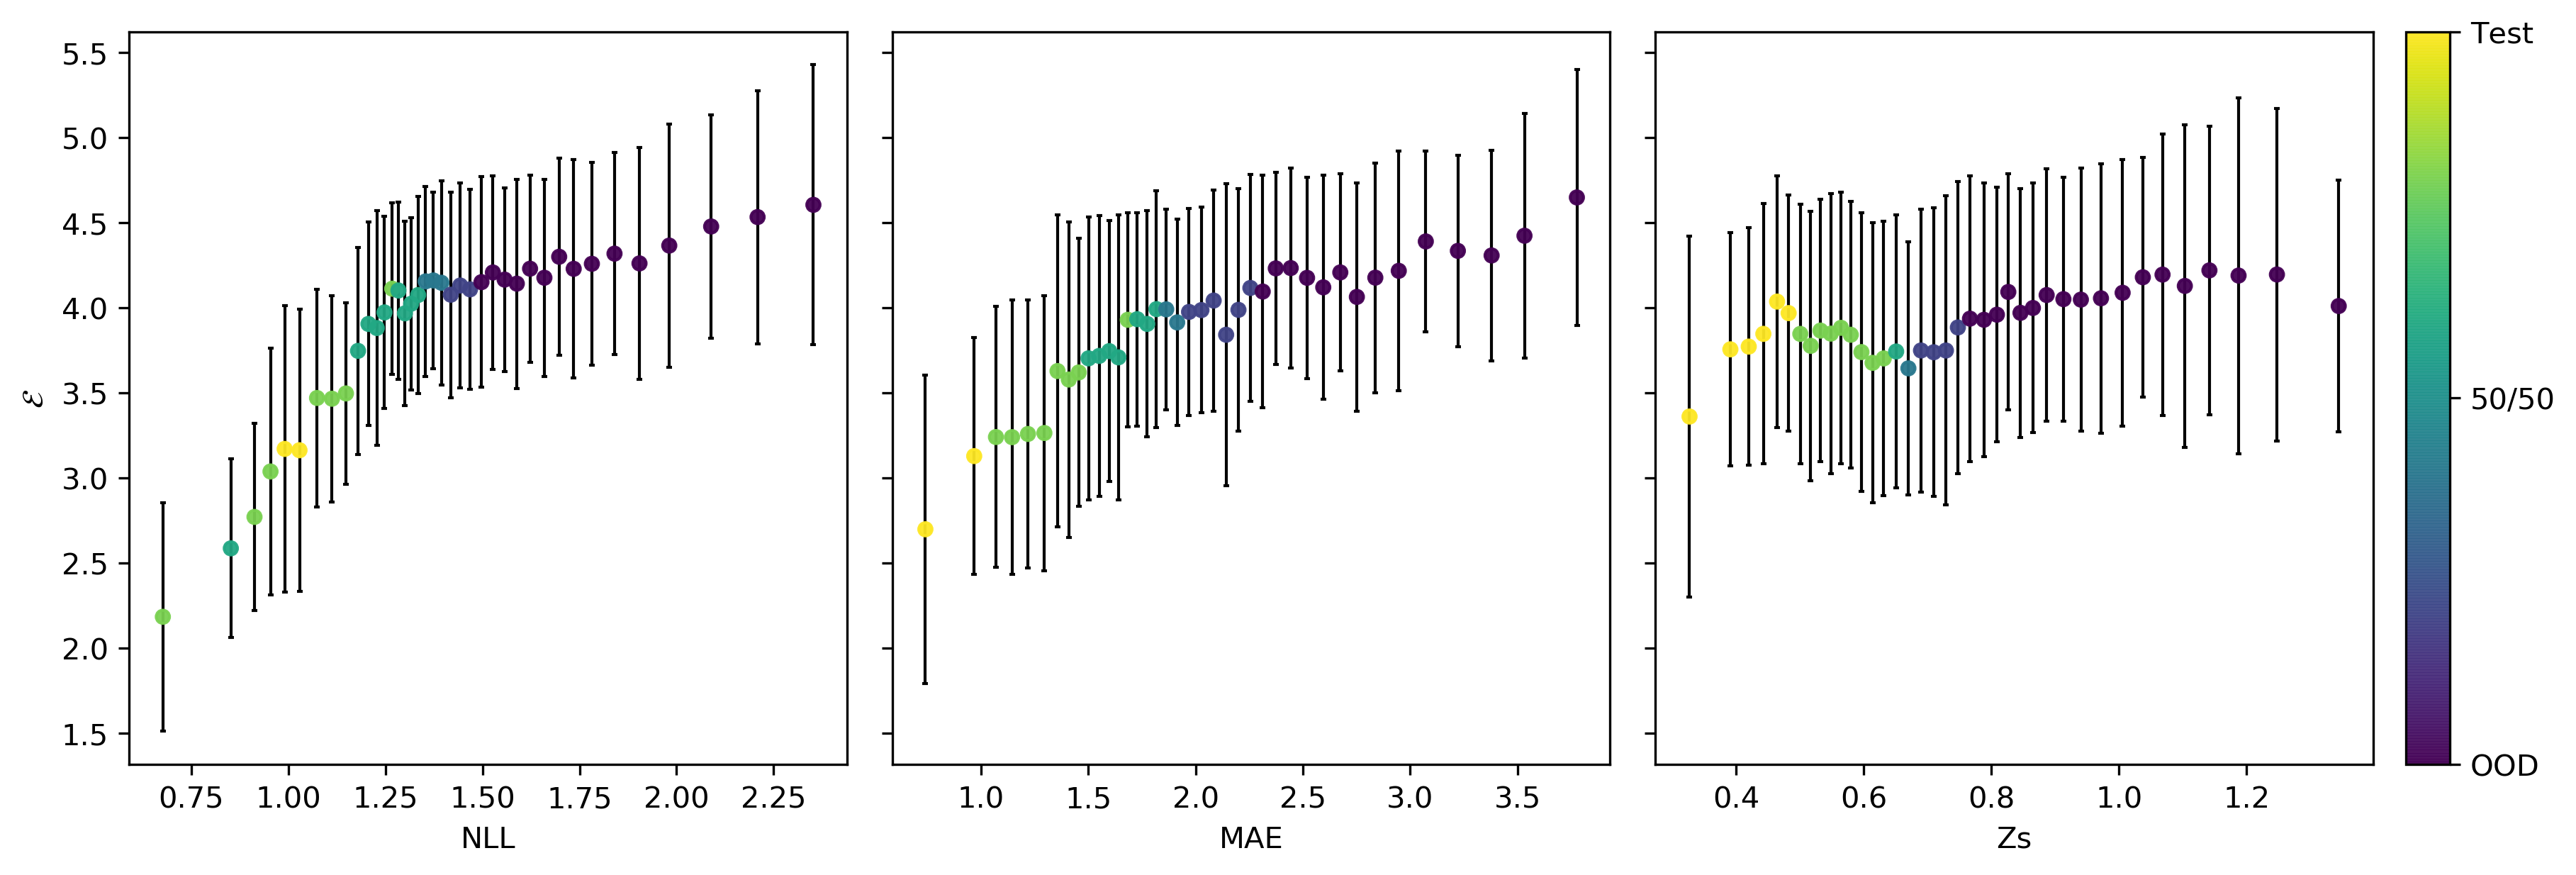
\includegraphics[width=\textwidth]{Experiments/figs/binned/revs_dropout_epistemic.png}
        \caption{Binned diagonal plots for the epistemic uncertainty.}
    \end{subfigure}
    
    \begin{subfigure}[b]{\textwidth}
        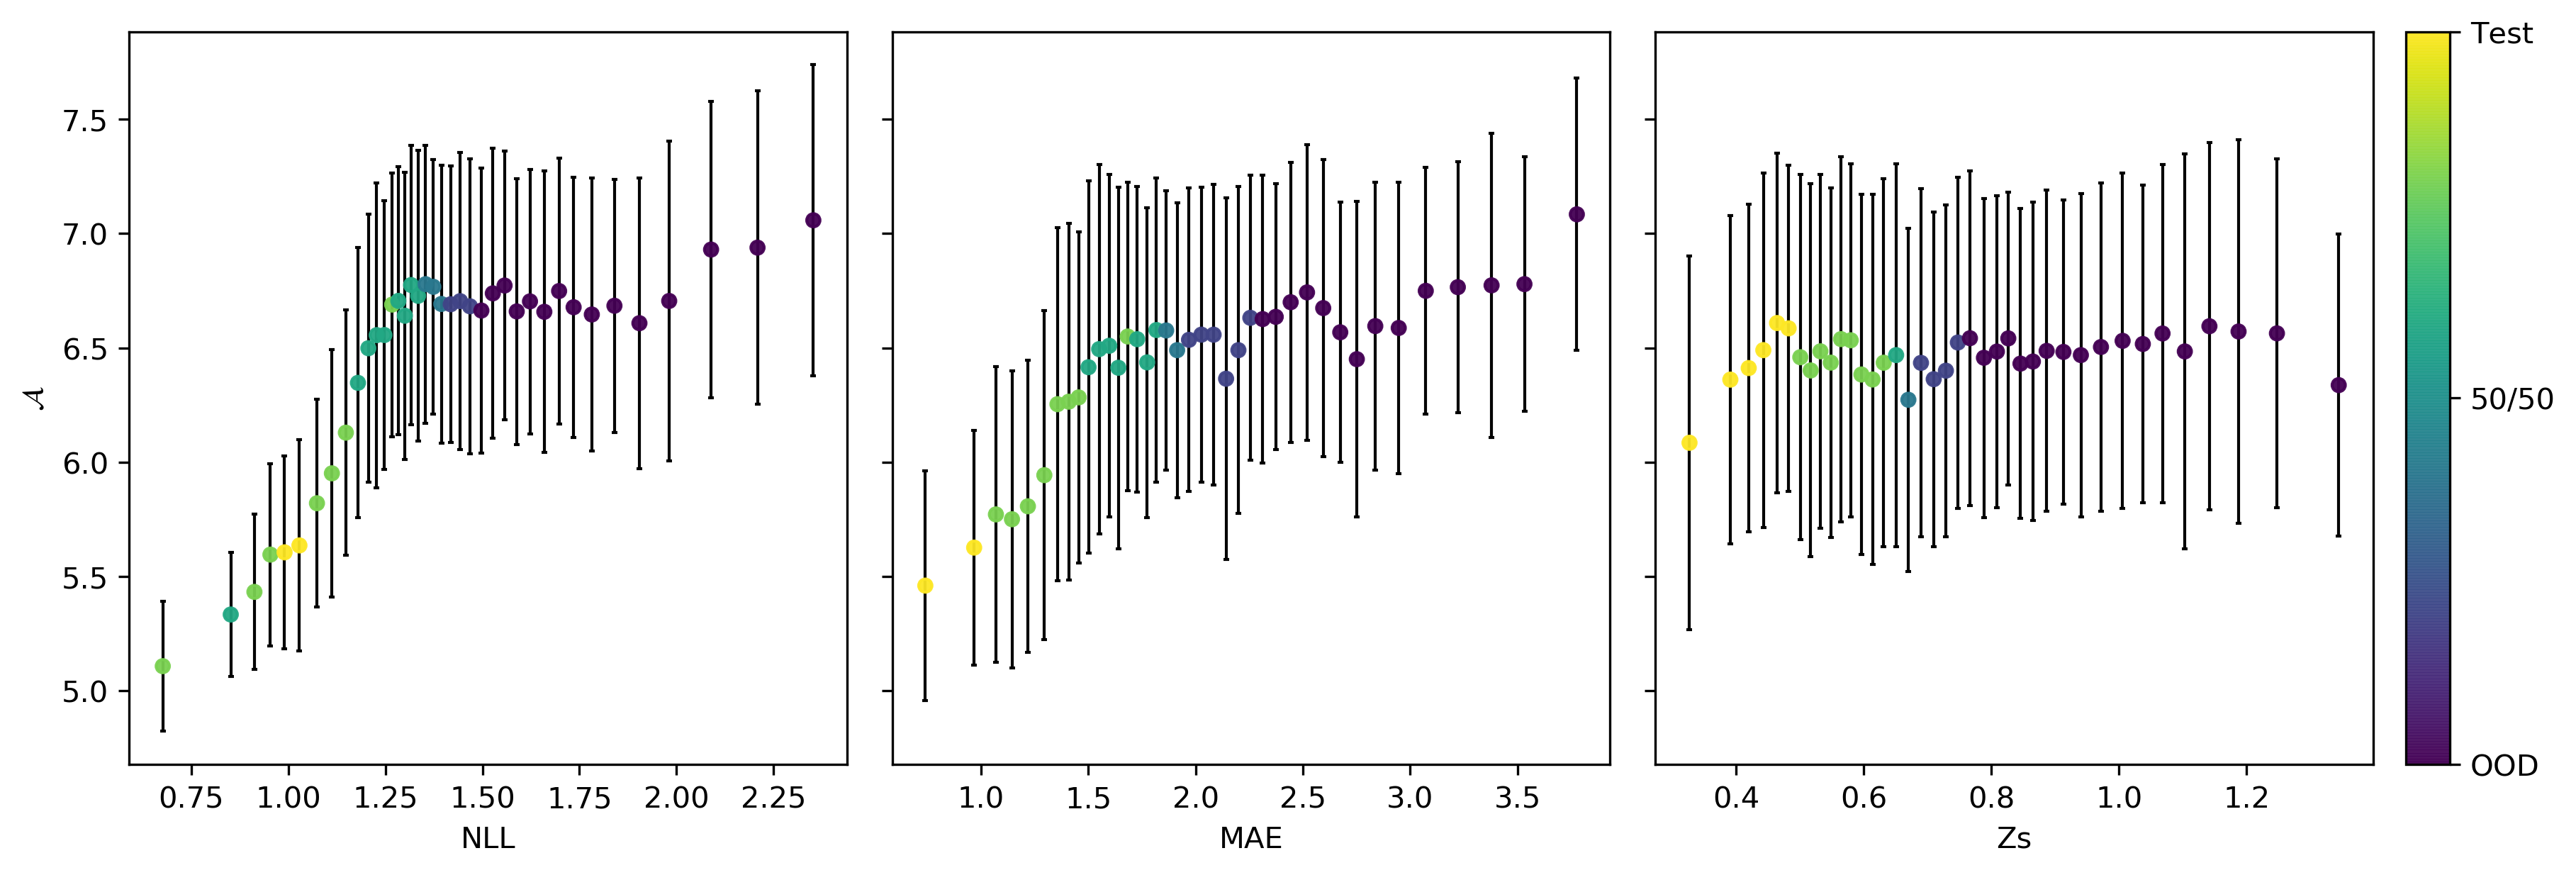
\includegraphics[width=\textwidth]{Experiments/figs/binned/revs_dropout_aleatoric.png}
        \caption{Binned diagonal plots for the aleatoric uncertainty.}
  \end{subfigure}
    \caption[Revs error-uncertainty diagonal plots for MC dropout]{Revs binned diagonal plots of the  uncertainty vs error scores(NLL, MAE, Z-score) over the combined splits(Test+OOD). The marker color denotes the ratio of test to OOD points in the bin.}
    \label{fig:revs_dropout_uncertainty_corr}
\end{figure}

\Cref{fig:revs_dropout_uncertainty_corr} shows binned diagonal plots of errors versus uncertainty for MC dropout. We can see that the two uncertainties behave roughly the same here. The plot shows that for low errors, the uncertainty increases with the error, but that correlation seems to fade as we move to higher error points. 


\subsection{Key points}

In this section, we will start by summarizing the key points from the in-depth results we just saw from our C-RNN model and MC dropout. Then we will show direct comparison of the key performance measures for the two models.

Our key findings 

\begin{itemize}
    \item The epistemic uncertainty estimated by the C-RNN model is effective in discriminating between in and out-of-distribution samples.
    
    \item The epistemic uncertainty estimated by MC dropout is not effective in discriminating between in and out-of-distribution samples.
    
    \item The aleatoric uncertainty behaves similarly in both models and is not effective in discriminating between the in and out-of-distribution samples.
    
    \item For the C-RNN model the epistemic and aleatoric uncertainties are not correlated and provide different types of information.
    
    \item For the MC dropout model the epistemic and aleatoric uncertainties are highly correlated and provide the same information. 
\end{itemize}{}


\begin{table*}[htbp]
\centering
    \begin{tabular}{l l c c c c c}  
        \toprule
        Model & split & MAE & NLL & $\rho$(MAE vs $\mathcal{E}$) &
        $\rho$(Z-score vs $\mathcal{E}$) & AUROC($\mathcal{E}$)\\
        \midrule
        \multirow{3}{*}{C-RNN} 
            & Test     & 0.55& 0.44 & 0.32  & 0.23 & - \\  
            & OOD      & 2.6 & 17.8 & 0.57  & 0.88 & -\\  
            & Test+OOD & 1.6 & 9.2  & 0.85  & 0.93 & 0.97\\ 

        \midrule
        \multirow{3}{*}{MC dropout} 
            & Test     & 1.26 & 1.14  & 0.36  & -0.06 & - \\  
            & OOD      & 2.55 & 1.62  & 0.32  & 0 & -\\  
            & Test+OOD & 1.8  & 1.38  & 0.42  & 0.1 & 0.64\\ 

        \toprule
    \end{tabular}
    \caption[Revs key results for comparison of C-RNN and MC dropout]{Revs key results for comparison of C-RNN and MC dropout. $\rho$ is the Pearson correlation.}
    \label{tbl:revs_comparison}
\end{table*}


\Cref{tbl:revs_comparison} contains a summary of the key results for comparison between C-RNN and MC dropout. The main difference between the two models is the approach to estimating the epistemic uncertainty. We can see that C-RNN's epistemic uncertainty performs significantly better in discriminating between the in and out-of-distribution points with an AUROC of 0.97 compared to MC dropout's 0.64.

Looking at how the uncertainty correlates with the errors, we can see that over the combined splits C-RNN performs better for both the MAE and the Z-score. C-RNN's epistemic uncertainty has an 0.93 correlation with the Z-score while MC dropout has a correlation of 0.1. Over the test split alone MC dropout shows a correlation of 0.32 between the epistemic uncertainty and the MAE, and -0.06 between the epistemic uncertainty and the Z-score. On the other hand, C-RNN shows a correlation of 0.32 between the epistemic uncertainty and the MAE, and 0.23 between the epistemic uncertainty and the Z-score. Thus even in the setting where OOD data is excluded C-RNN's epistemic uncertainty correlates better with the Z-score.    
 



\subsubsection{Ablations}

\begin{table*}[htbp]
\centering
    \begin{tabular}{l l c c c c }  
        \toprule
        Model & split & MAE & NLL & $\rho$(MAE vs $\mathcal{E}$) &
        $\rho$(Z-score vs $\mathcal{E}$)\\
        \midrule
        \multirow{3}{*}{C-RNN(no annealing)} 
            & Test     & 0.69 & 0.63 & 0.48  & 0.15\\  
            & OOD      & 3.07 & 9.91 & 0.58  & 0.44\\  
            & Test+OOD & 1.9  & 5.2  & 0.66  & 0.59\\ 

        \midrule
        \multirow{3}{*}{C-RNN(no weighting)} 
            & Test     & 0.55 & 0.42  & 0.48  & 0.2\\  
            & OOD      & 2.51 & 7.66  & 0.42  & 0.4 \\  
            & Test+OOD & 1.6  & 4.04  & 0.77  & 0.77\\ 
            
        \midrule
        \multirow{3}{*}{C-RNN} 
            & Test     & 0.55& 0.44 & 0.32  & 0.23\\  
            & OOD      & 2.6 & 17.8 & 0.57  & 0.88\\  
            & Test+OOD & 1.6 & 9.2  & 0.85  & 0.93\\ 

        \toprule
    \end{tabular}
    \caption{Revs ablation study for C-RNN}
    \label{tbl:revs_ablation}
\end{table*}


Our last set of results with the Revs dataset is going to be an ablation study, showing the effect of the additional components we use to train C-RNN, namely the KL annealing and the compression loss weighting. 

In \cref{tbl:revs_ablation} we show the key results for our full C-RNN model versus ablated versions. We show two ablated versions of the model one trained without the KL annealing and one trained without the compression loss weighting, along with the our full model.

Recall our motivation for adding the KL annealing to our model is to prevent a form of under-fitting caused by the model trying to minimize the penalty of encoding information in the latent state. In the top part of \cref{tbl:revs_ablation} we show the performance of C-RNN trained without KL annealing. We can see that the test MAE is higher with 0.69 versus 0.55 for the standard full C-RNN. The correlation of the epistemic uncertainty with the errors is also lower. For instance the correlation with the Z-score is 0.59 for the combined split, whereas the full model has a correlation of 0.93 in that setting. 

In the middle part of the model we have the results for a C-RNN trained without our compression loss weighting scheme. Recall that we introduced this scheme to increase the correlation between the epistemic uncertainty and the Z-score. We can see from the table that this is exactly what happens with the standard model having a correlation of 0.93 between the epistemic uncertainty and the Z-score, the model trained without the weighting scheme has a correlation of 0.77. 




With this ablation study we conclude our in-depth analysis and work on the revs dataset. In the next section we will present result using a different dataset in order to further validate the findings and insights we presented in this section. 